\section*{Mapping 2D array to 1D array in \texttt{C}}
\begin{itemize}
\item given a grid of size $M$ by $N$ where $M$ is row $\#$ and $N$ is column $\#$
\item halo layer around only 4 edges: top, bottom, left, right
\item corner elements of halo: (0,0), (0,$N+1$), ($M+1$,$N+1$), ($M+1$,0)
\item corner elements of interior field: (1,1), (1,$N$), ($M,N$), ($M$,1)
\item using 1D array \texttt{u[]} to store all points, thus \texttt{u} size $(M+2)\times(N+2)$
\item parallel algorithm implementation on $P$ by $Q$ process grid
\item use a 2-stage halo exchange: top-bottom then left-right
\end{itemize}
% M by N matrix
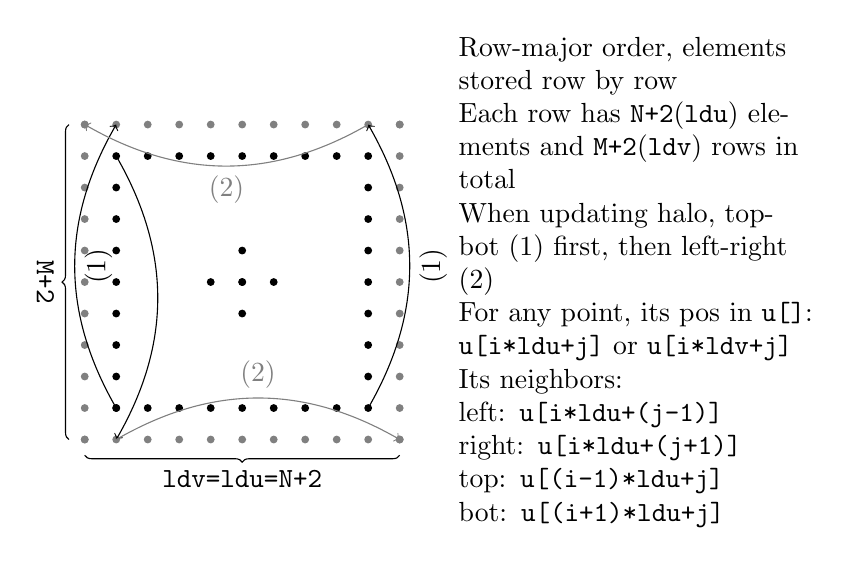
\begin{tikzpicture}
  [halo/.style={circle,fill,gray,inner sep=1pt},
  innr/.style={circle,fill,inner sep=1pt},
  info/.style={inner sep=1ex,font=\small}]

  % halo
  \foreach \i in {0,0.4,...,4} {
    \node at (\i,0)[halo]{}; %halo top
    \node at (\i,4)[halo]{}; %halo bot
    \node at (0,\i)[halo]{}; %halo left
    \node at (4,\i)[halo]{}; %halo right
  }

  % halo
  \foreach \j in {0.4,0.8,...,3.6} {
    \node at (\j,3.6)[innr]{}; %inner top
    \node at (\j,0.4)[innr]{}; %inner bot
    \node at (0.4,\j)[innr]{}; %inner left
    \node at (3.6,\j)[innr]{}; %inner right
  }
  \node at (3.6,3.6)[innr]{};

  \foreach \m in {1.6,2.0,2.4} {
    \node at (\m, 2.0)[innr]{};
    \node at (2.0, \m)[innr]{};
  }

  % neighbors

  \draw[decorate,decoration={brace,mirror}] (-.2,4.0) -- (-.2,0); %left
  \draw[decorate,decoration={brace,mirror}] (0,-.2) -- (4.0,-.2); %bot
  \node at (-.5,2)[rotate=-90]{\texttt{M+2}};
  \node at (2,-.5)[](ldu){\texttt{ldv=ldu=N+2}};

  % halo src to dest
  \path[->] (0.4,0.4) edge[bend left] node[below,sloped]{(1)} (0.4,4); %top halo left
  \path[->] (3.6,0.4) edge[bend right] node[below,sloped]{(1)} (3.6,4);%top halo right
  \path[->] (0.4,3.6) edge[bend left] (0.4,0);

  \path[->] (3.6,4) edge[bend left,gray] node[below,sloped]{(2)} (0,4);
  \path[->] (0.4,0) edge[bend left,gray] node[above,sloped]{(2)} (4,0);

  % txt
  \node[xshift=7cm,yshift=2cm,text width=4.5cm]
  {
    Row-major order, elements stored row by row\\
    Each row has \texttt{N+2}(\texttt{ldu}) elements and \texttt{M+2}(\texttt{ldv}) rows in total\\
    When updating halo, top-bot (1) first, then left-right (2) \\
    For any point, its pos in \texttt{u[]}:
    \texttt{u[i*ldu+j]} or \texttt{u[i*ldv+j]}\\
    Its neighbors:\\
    left:  \texttt{u[i*ldu+(j-1)]} \\
    right: \texttt{u[i*ldu+(j+1)]}\\
    top:   \texttt{u[(i-1)*ldu+j]}\\
    bot:   \texttt{u[(i+1)*ldu+j]}
  };
\end{tikzpicture}
      % top left halo, \texttt{u[1] = u[(M+1)*ldu+1]}\\
      % top right halo, \texttt{u[1] = u[(M+1)*ldu+1]}\\
      % bot left halo, \texttt{u[1] = u[(M+1)*ldu+1]}\\
      % bot right halo, \texttt{u[1] = u[(M+1)*ldu+1]}\\
      % left halo, \texttt{u[1] = u[(M+1)*ldu+1]}\\
      % right halo, \texttt{u[1] = u[(M+1)*ldu+1]}\\
